\documentclass[11pt]{article}
\usepackage{cite}

\usepackage{hyperref}
%biblio
\usepackage{natbib}
\usepackage{url}
\usepackage{wrapfig}

%Math
\usepackage{amsmath}
\usepackage{amsfonts}
\usepackage{amssymb}
\usepackage{amsthm}
\usepackage{ulem}
\usepackage{bm}
\usepackage{stmaryrd} %f\UTF{00FC}r Blitz!

%PageStyle
%\usepackage[ngerman]{babel} % deutsche Silbentrennung1
\usepackage[utf8x]{inputenc} 
\usepackage{fancyhdr, graphicx}
\usepackage{subcaption}
\usepackage[scaled=0.92]{helvet}
\usepackage{enumitem}
\usepackage{parskip}
\usepackage[a4paper,top=2cm]{geometry}
\setlength{\textwidth}{17cm}
\setlength{\oddsidemargin}{-0.5cm}
\usepackage{lastpage} % for getting last page number
\renewcommand{\familydefault}{\sfdefault}
\usepackage{setspace}
\usepackage{acronym}


% Code listenings
\usepackage{color}
\usepackage{xcolor}
\usepackage{listings}
\usepackage[font=it]{caption}
\DeclareCaptionFont{white}{\color{white}}
\DeclareCaptionFormat{listing}{\colorbox{gray}{\parbox{\textwidth}{#1#2#3}}}
\captionsetup[lstlisting]{format=listing,labelfont=white,textfont=white}
\lstset{
 language=Java,
 basicstyle=\footnotesize\ttfamily, % Standardschrift
 numbers=left,               % Ort der Zeilennummern
 numberstyle=\tiny,          % Stil der Zeilennummern
 stepnumber=1,              % Abstand zwischen den Zeilennummern
 numbersep=5pt,              % Abstand der Nummern zum Text
 tabsize=2,                  % Groesse von Tabs
 extendedchars=true,         %
 breaklines=true,            % Zeilen werden Umgebrochen
 frame=b,         
 %commentstyle=\itshape\color{LightLime}, Was isch das? O_o
 %keywordstyle=\bfseries\color{DarkPurple}, und das O_o
 basicstyle=\small,
 stringstyle=\color[RGB]{42,0,255}\ttfamily, % Farbe der String
 keywordstyle=\color[RGB]{127,0,85}\ttfamily, % Farbe der Keywords
 commentstyle=\color[RGB]{63,127,95}\ttfamily, % Farbe des Kommentars
 showspaces=false,           % Leerzeichen anzeigen ?
 showtabs=false,             % Tabs anzeigen ?
 xleftmargin=17pt,
 framexleftmargin=17pt,
 framexrightmargin=5pt,
 framexbottommargin=4pt,
 showstringspaces=false      % Leerzeichen in Strings anzeigen ?        
}

\usepackage{xcolor}

%Config
\fancypagestyle{firststyle}{ %Style of the first page
 \fancyhf{}
 \fancyheadoffset[L]{0.6cm}
 \lhead{
 
\includegraphics[scale=0.8]{./fhnw_ht_e_10mm.jpg}}
 \renewcommand{\headrulewidth}{0pt}
 \lfoot{Institute 4 Data Science,\linebreak www.fhnw.ch }
}

\fancypagestyle{documentstyle}{ %Style of the rest of the document
 \fancyhf{}
 \fancyheadoffset[L]{0.6cm}
\lhead{
 
\includegraphics[scale=0.8]{./fhnw_ht_e_10mm.jpg}}
 \renewcommand{\headrulewidth}{0pt}
 \lfoot{P9 Distributed Image Reconstruction for new Radio Interferometers}
 \rfoot{\thepage\ / \pageref{LastPage} }
}

\fancypagestyle{tableofcontent}{ %Style of the rest of the document
 \fancyhf{}
 \fancyheadoffset[L]{0.6cm}
\lhead{
 
\includegraphics[scale=0.8]{./fhnw_ht_e_10mm.jpg}}
 \renewcommand{\headrulewidth}{0pt}
 \cfoot{\thepage}
}

\fancypagestyle{abstract}{ %Style of the first page
 \fancyhf{}
 \fancyheadoffset[L]{0.6cm}
 \lhead{
 
\includegraphics[scale=0.8]{./fhnw_ht_e_10mm.jpg}}
 \renewcommand{\headrulewidth}{0pt}
 \cfoot{}
}


%Metadata
\numberwithin{equation}{section}

\newlength{\twosubht}
\newsavebox{\twosubbox}

\begin{document}
\title{P9 Distributed Image Reconstruction for the new Radio Interferometers}
\author{Jonas Schwammberger}
\date{\today}

\section*{Distributed Image Reconstruction for Radio Interferometers}
In Astronomy, instruments with higher angular resolution allows us to measure ever smaller structures in the sky. For Radio frequencies, the angular resolution is bound to the antenna dish diameter, which puts practical and financial limitations on the highest possible angular resolution. Radio Interferometers get around this limitation by using several smaller antennas instead. Together, they act as a single large antenna with higher angular resolution at lower financial costs compared to single dish instruments.

Each antenna pair of an Interferometer measures a single Fourier component of the observed image. We can retrieve the image by calculating the Fourier Transform of the measurements. However, since the Interferometer only measures an incomplete set of Fourier components, the resulting image is "dirty", convolved with a Point Spread Function ($PSF$). Calculating the Fourier Transform is not enough. To reconstruct the from an Interferometer image, an algorithm has to find the observed image with only the dirty image and the $PSF$ as input. It has to perform a deconvolution. The difficulty lies in the fact that there are potentially many valid deconvolutions for a single measurement, and the algorithm has to decide for the most likely one. How similar the truly observed image and the reconstructed images are depends largely on the deconvolution algorithm.

State-of-the-art image reconstructions use the Major Cycle architecture (shown in Figure \ref{hypo:major3}), which contains three operations: Gridding, FFT and Deconvolution.

\begin{figure}[h]
	\centering
	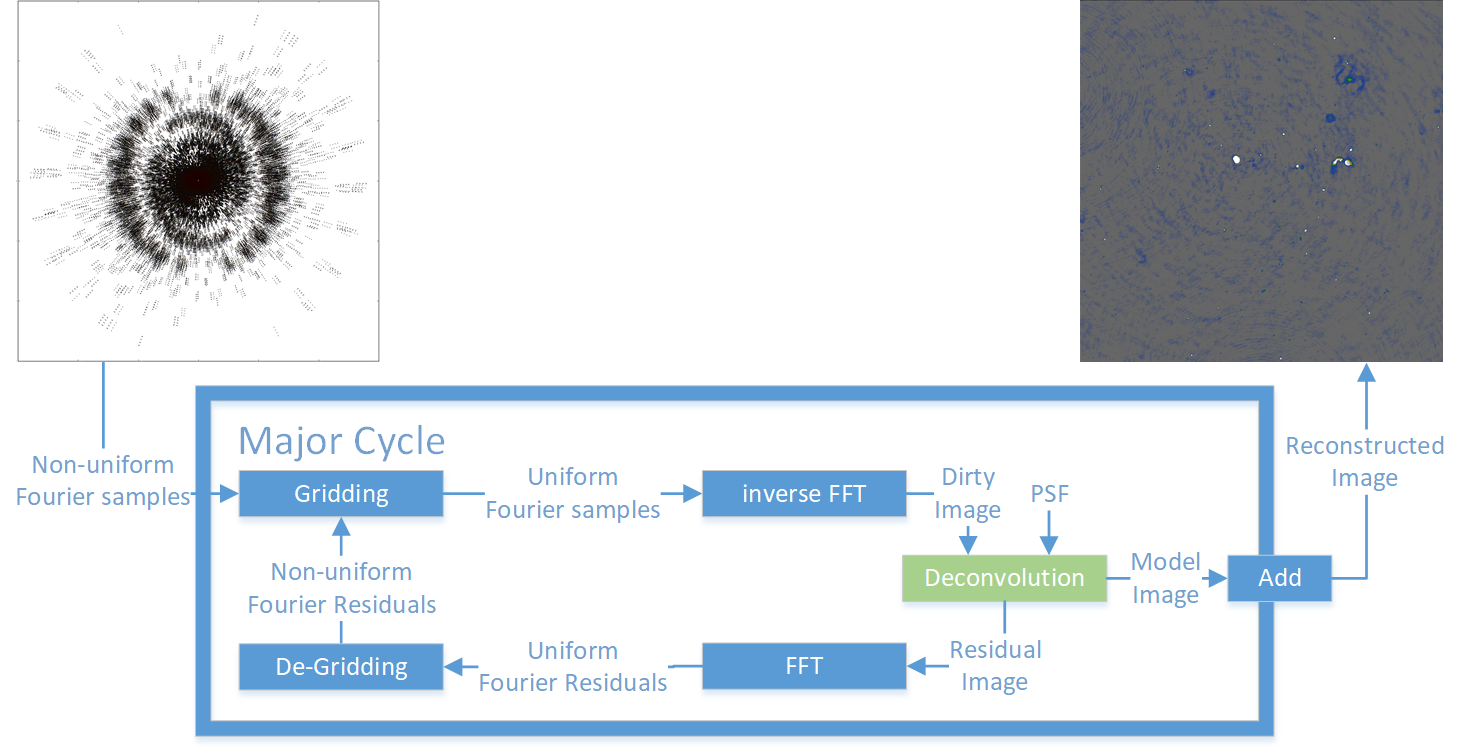
\includegraphics[width=0.80\linewidth]{./Major-Minor3.png}
	\caption{The Major Cycle Architecture of image reconstruction algorithms}
	\label{hypo:major3}
\end{figure}

The first operation in the Major Cycle, Gridding, takes the non-uniformly sampled Fourier measurements from the Interferometer and interpolates them on a uniformly spaced grid. The uniform grid lets us use FFT to calculate the inverse Fourier Transform and we arrive at the dirty image. A deconvolution algorithm takes the dirty image plus the $PSF$ as input, producing the deconvolved "model image", and the residual image as output. At this point, the reverse operations get applied to the residual image. First the FFT and then De-gridding, arriving at the non-uniform Residuals. The next Major Cycle begins with the non-uniform Residuals as input. The cycles are necessary, because the Gridding and Deconvolution operations are only approximations. Over several cycles, we reduce the errors introduced by the approximate Gridding and Deconvolution. The final, reconstructed image is the addition of all the model images of each Major Cycle. 

\subsection*{The case for distributed Reconstruction}*
New Interferometer produce an ever increasing number of measurements, creating ever larger reconstruction problems. A single image can contain several terabytes of Fourier measurements. Handling reconstruction problems of this size forces us to use distributed computing. However, state-of-the-art Gridding and Deconvolution algorithms only allow for limited distribution. How to scale the Gridding and Deconvolution algorithms to large problem sizes is still an open question.

Recent developments make a distributed Gridder and a distributed Deconvolution algorithm possible. Veeneboer et al\cite{veenboer2017image} found an input partitioning scheme, which allowed them to perform the Gridding on the GPU. The same partitioning scheme can potentially be used to distribute the Gridding onto multiple machines. For Deconvolution, there exist parallel implementations for certain algorithms like MORESANE\cite{dabbech2015moresane}. These can be used as a basis for a fully distributed image reconstruction.

In this project, we want to make the first steps towards an image reconstruction algorithm, which is distributed from end-to-end, from Gridding up to and including deconvolution. We create our own distributed Gridding and Deconvolution algorithms, and analyse the bottlenecks that arise.

\subsection*{First steps towards a distributed Algorithm}
In this project, we make the first steps towards a distributed Major Cycle architecture (shown in figure \ref{hypo:major3}) implemented C\#. We port Veeneboer et al's Gridder, which is written in C++, to C\# and modify it for distributed computing. We implement a simple deconvolution algorithm based on the previous project and create a first, non-optimal distributed version of it.

In the next step, we create a more sophisticated deconvolution algorithm based on the shortcomings of the first implementation. We use simulated and real-world observations of the MeerKAT Radio Interferometer and measure its speed up. We identify the bottlenecks of the current implementation and explore further steps.

From the first lessons, we continually modify the distributed algorithm and focus on decreasing the need for communication between the nodes, and increase the overall speed up compared to single-machine implementations. Possible Further steps:
\begin{itemize}
	\item Distributed FFT
	\item Replacing the Major Cycle Architecture
	\item GPU-accelerated Deconvolution algorithm.
\end{itemize}

A state-of-the-art reconstruction algorithm has to correct large number of measurement effects arising from the Radio Interferometer. Accounting for all effects is out of the scope for this project. We make simplifying assumptions, resulting in a proof-of-concept algorithm.

\newpage
\bibliography{mybib}{}
%\bibliographystyle{plain}
\bibliographystyle{unsrt}

\end{document}